% 2019-02-25

% See presentation for GCSC class https://docs.google.com/presentation/d/12naRTrTU_b9B7hangRKMeVa-7t6DDiWBFSIuVOw7Xvk/edit?usp=sharing

\documentclass[10pt]{article}
\usepackage[T1]{fontenc}
\usepackage{amssymb}
\usepackage{amsmath}
\usepackage{graphicx}
% \begin{figure}[h]
% \centering
% \includegraphics[width=6.5in]{folder/photo.png}
% \caption{}
% \label{}
% \end{figure}



\usepackage{tikz}
\usetikzlibrary{arrows}
\usepackage{subfigure}
\usepackage{stackrel}
\usepackage{blindtext}

\usepackage[url=false]{biblatex}
\addbibresource{library.bib}

\oddsidemargin=0.15in
\evensidemargin=0.15in
\topmargin=-.5in
\textheight=9in
\textwidth=6.25in

\usepackage[colorlinks=true,breaklinks,pdfpagemode=none,linkcolor=blue,citecolor=blue]{hyperref}

\usepackage{enumerate}
% \vspace{-6pt}
% \begin{itemize}
%     \setlength{\itemsep}{0pt}%
%     \setlength{\parskip}{0pt}%
%     \item Item 1
%     \item Item 2
%         \begin{itemize}
%             \setlength{\itemsep}{0pt}%
%             \setlength{\parskip}{0pt}%
%             \item Sublist Item 1
%             \item Sublist Item 2
%         \end{itemize}
%         \item Item 3
% \end{itemize}
% \vspace{-6pt}


\usepackage{enumitem}
\setlist{itemsep=0mm}

\usepackage{amsmath,amsfonts,amssymb,bm}


\begin{document}

   \noindent
   \begin{center}

   \hrulefill
   
   \vspace{5pt}
   
   \makebox[\textwidth]{ {\bf Energy Systems Analysis} \hfill  A.D. Smith 2019}
   \vspace{0pt}
   
   {\Large \hfill  Lecture 18. Building Energy Use: Quantifying Emissions and Water Use}
   \vspace{5pt}
   
 {\color{darkgray}{\center{ \small{      ``Given the increased urgency in curbing global greenhouse gas emissions, reducing the carbon footprint of new and existing buildings has become a priority in many jurisdictions.''
\\%[3pt]
\rightline{{\rm --- Brackney, Parker, Macumber, and Benne \cite{OpenStudio-book}}}}}}}
  
   \hrulefill
   \end{center}



\section{Emissions reduction}

When discussing emissions reductions, it's important to clarify what exactly you are interested in reducing and why. A building may be responsible for emissions of $CO_2$, ($N_2O$), or $PM_{2.5}$, but cutting $CO_2$ emissions in half is not the same thing as cutting $PM_{2.5}$ emissions in half. It's also not necessarily going to halve the building's carbon footprint.

Greenhouse gases (GHGs) contribute to global climate change, including carbon dioxide ($CO_2$), methane ($CH_4$), nitrous oxide $N_2O$, chlorofluorocarbons (e.g. Freon) and hydrochlorofluorocarbons \cite{Epa2014-mz}. Their relative impact on global warming can be gauged with their \textbf{global warming potential} (GWP), which ``is a measure of how much energy the emissions of 1 ton of a gas will absorb over a given period of time, relative to the emissions of 1 ton of carbon dioxide ($CO_2$).'' \cite{Epa2017-ur}

Local air quality is affected by a number of substances, including some emitted due to human activity in the built environment. Notably, \textbf{criteria pollutants} are those that the U.S. Environmental Protection Agency (EPA) uses to set quantitative standards for air quality: ground-level ozone ($O_3$), particulate matter ($PM$), carbon monoxide ($CO$), lead, sulfur dioxide ($SO_2$), nitrogen dioxide ($NO_2$) \cite{Epa2014-xv}.

\subsection{Direct}

\textbf{Direct} emissions are those that occur at the site. These are probably the first emissions you think of when imagining a given building, and they may be prioritized if the building's impact on local air quality is a significant concern.

These are also called \textbf{Scope 1} emissions within the Greenhouse Gas Protocol framework published by the World Resources Institute: ``GHG emissions from sources located within
the [site] boundary.'' \cite{ghgprotocol2014}


\subsection{Indirect}

\textbf{Indirect}, or off-site, emissions are those that occur elsewhere but are caused or impacted by a building's operation. An example would be emissions occurring at a power plant that is burning fuel miles away while providing grid electricity that's purchased to provide services at a building site. They may be prioritized if the building's impact on greenhouse gas emissions is a significant concern.

These are also called \textbf{Scope 2} emissions within the Greenhouse Gas Protocol framework: ``GHG emissions occurring as a consequence  of the use of grid-supplied electricity, heat, 
steam and/or cooling within the [site] boundary.'' \cite{ghgprotocol2014}

For a quick estimate of the indirect emissions associated with electricity purchases in a U.S. location, visit Power Profiler at \url{https://www.epa.gov/energy/power-profiler} and enter your zip code.

\subsubsection{Flat rate emission factors}

The most straightforward option for calculating indirect emissions to due electricity purchases is to use a simple flat rate emissions factor that gives one number for the amount of emissions per unit of electrical energy (e.g. lb/MWh). Power Profiler will show these numbers for $CO_2$, $SO_2$, and $NO_x$, and you can simply multiply by each MWh of electricity used to get an estimate for indirect emissions based on the region they've aggregated. Our eGRID subregion is WECC Northwest \cite{eGRIDsupportdoc2016}, abbreviated NWPP (for Northwest Power Pool), as shown in Figure \ref{egr}. You may recall from Lecture 3 that this larger region is not necessarily representative of Utah's power generation mix; for instance, it includes a significant portion of hydropower generation. You could also make your own estimate based on Utah's fuel mix (see Figure \ref{sankeyUT}); while there's no guarantee that electricity produced within the state will be consumed within the state (we are a net power exporter), this would be a little more representative of the fuel mix contributing to power purchased here compared with using the fuel mix for NWPP as a whole.



            \begin{figure}[h]
      %      \centering
            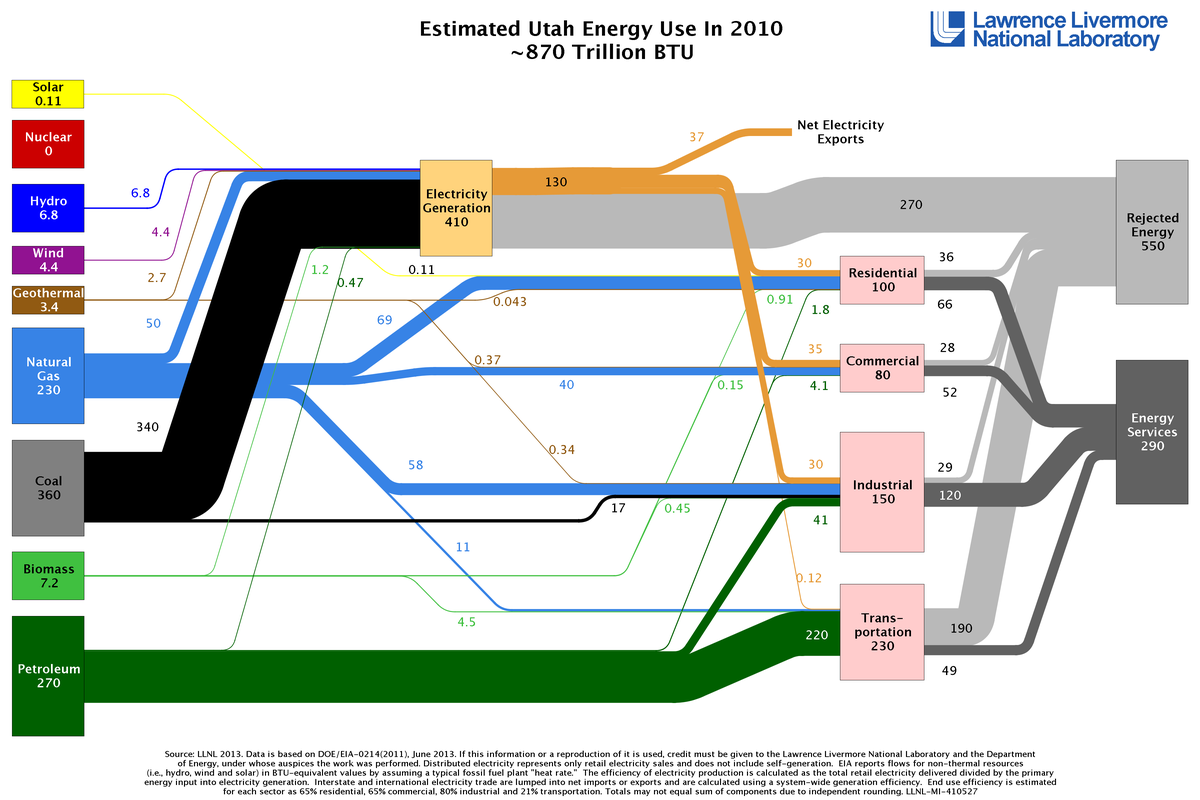
\includegraphics[width=6.5in]{extras18/sankey_UT.png}
            \caption{Utah energy flow chart for 2011 from LLNL \cite{noauthor_undated-zv}}
            \label{sankeyUT}
            \end{figure}



This is quick and easy to implement, but doesn't capture anything about how emissions vary with time of use or location of use. If you use power disproportionately at peak or off-peak hours, or if you happen to be located in an area within the grid topology where electricity tends to be mostly generated by coal or mostly generated by renewables, this may give you an inaccurate picture of your ``actual'' emissions. It's not possible to account for your true emissions with certainty because it's not possible to physically trace a quantity of electrical energy to exact generators---we make a statistical best estimate.


\begin{figure}[h]
\centering
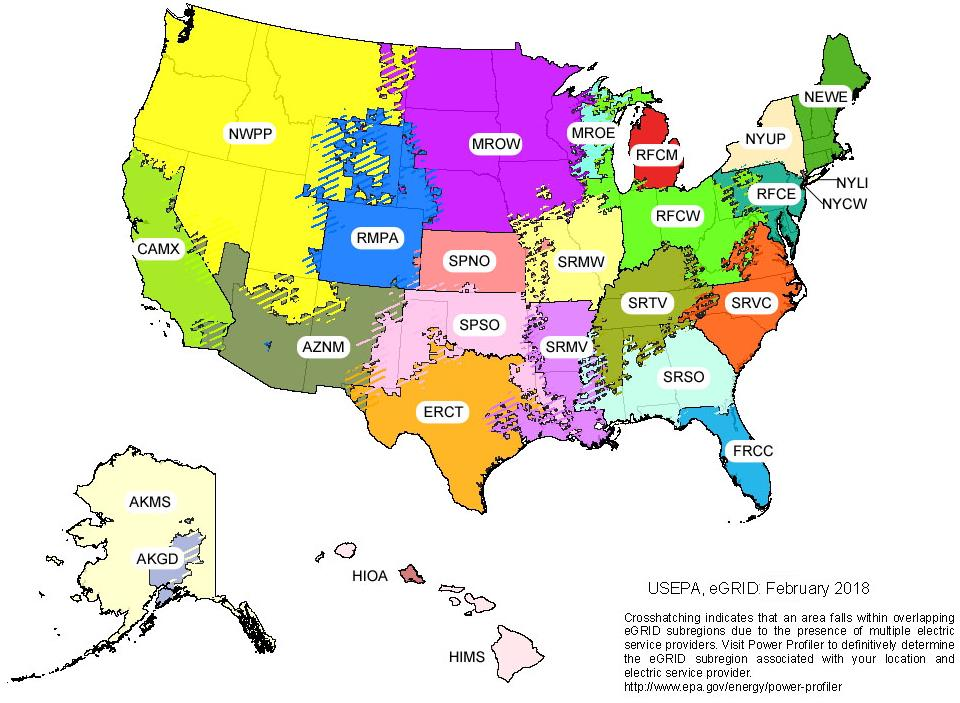
\includegraphics[width=5in]{extras18/egridFeb2018.jpg}
\caption{Representational map of the boundaries of eGRID subregions  \cite{eGRIDsupportdoc2016}}
\label{egr}
\end{figure}



\subsubsection{Time-varying, regionally aggregated emission factors}

Another option that's fairly straightforward to implement, but begins to capture some of the temporal variability in emissions from grid generators, is to use the Hourly Energy Emission Factors for Electricity Generation in the United States published by the National Renewable Energy Laboratory (NREL) and based on Environmental Protection Agency (EPA) data \cite{EPAfactors}. You may also recall these from Lecture 5. The emissions are based on changes to which generators are producing power at a given time of day and a given time of year, based on previously recorded data \cite{eGRID} and economic models run using GridView software \cite{GridView}.

There are two major concerns with the accuracy of this method: (1) The data are still aggregated, which means the building is treated the same no matter where it is located physically and within the grid network; and (2) The factors are the result of modeling performed with proprietary software, using data collected from 2005--2008 \cite{EPAfactors}.


\subsubsection{Temporally and spatially resolved emission factors}

Finally, a technically preferred option, but one that's difficult to implement in practice, is to use real-time data about what generators are serving the load on the grid at a given time (or, in a simulation model, which generators would be expected to serve a given load at a given time). This requires data that often is not publicly available as well as computational resources. Please refer to the Lecture 5 slides and our related publication \cite{Fallahi2018SETA} for more about some of the methods that can be used to make this type of emissions quantification.

\subsection{Embodied emissions}

There are many reasons that emissions may be produced in conjunction with the manufacture and transportation of building components and with items we purchase and use day-to-day. These are called \textbf{Scope 3} emissions within the GHG Protocol: ``All other GHG emissions that occur outside
the [site] boundary as a result of activities
taking place within the [site] boundary.'' \cite{ghgprotocol2014}

As you can imagine, this is a difficult category to capture. The carbon footprinting exercise you did in Homework 1 was an attempt to look at $CO_2$ emissions holistically, including Scope 3 or `embodied' emissions. Embodied (or you may also see the word `embedded') indicates that the emissions are not readily apparent but that they should be accounted for within the environmental analysis of some product or service.  We'll talk more about this idea in Lecture 19.

\section{Water conservation}

Water use due to human activity can affect ecosystems, weather and climate, food production, and the ability of other humans to have enough fresh water now and in the future to meet their basic needs. However, the use of potable, or treated, water is a small portion of overall water use. Most water used worldwide \cite{noauthor_2015-ye} and in the U.S. \cite{EPAhowweusewater} is due to agriculture or power generation. If we continue to use water at current rates, we will face a water crisis---a severe deficit of available water to serve the world's population.


            \begin{figure}[h]
      %      \centering
            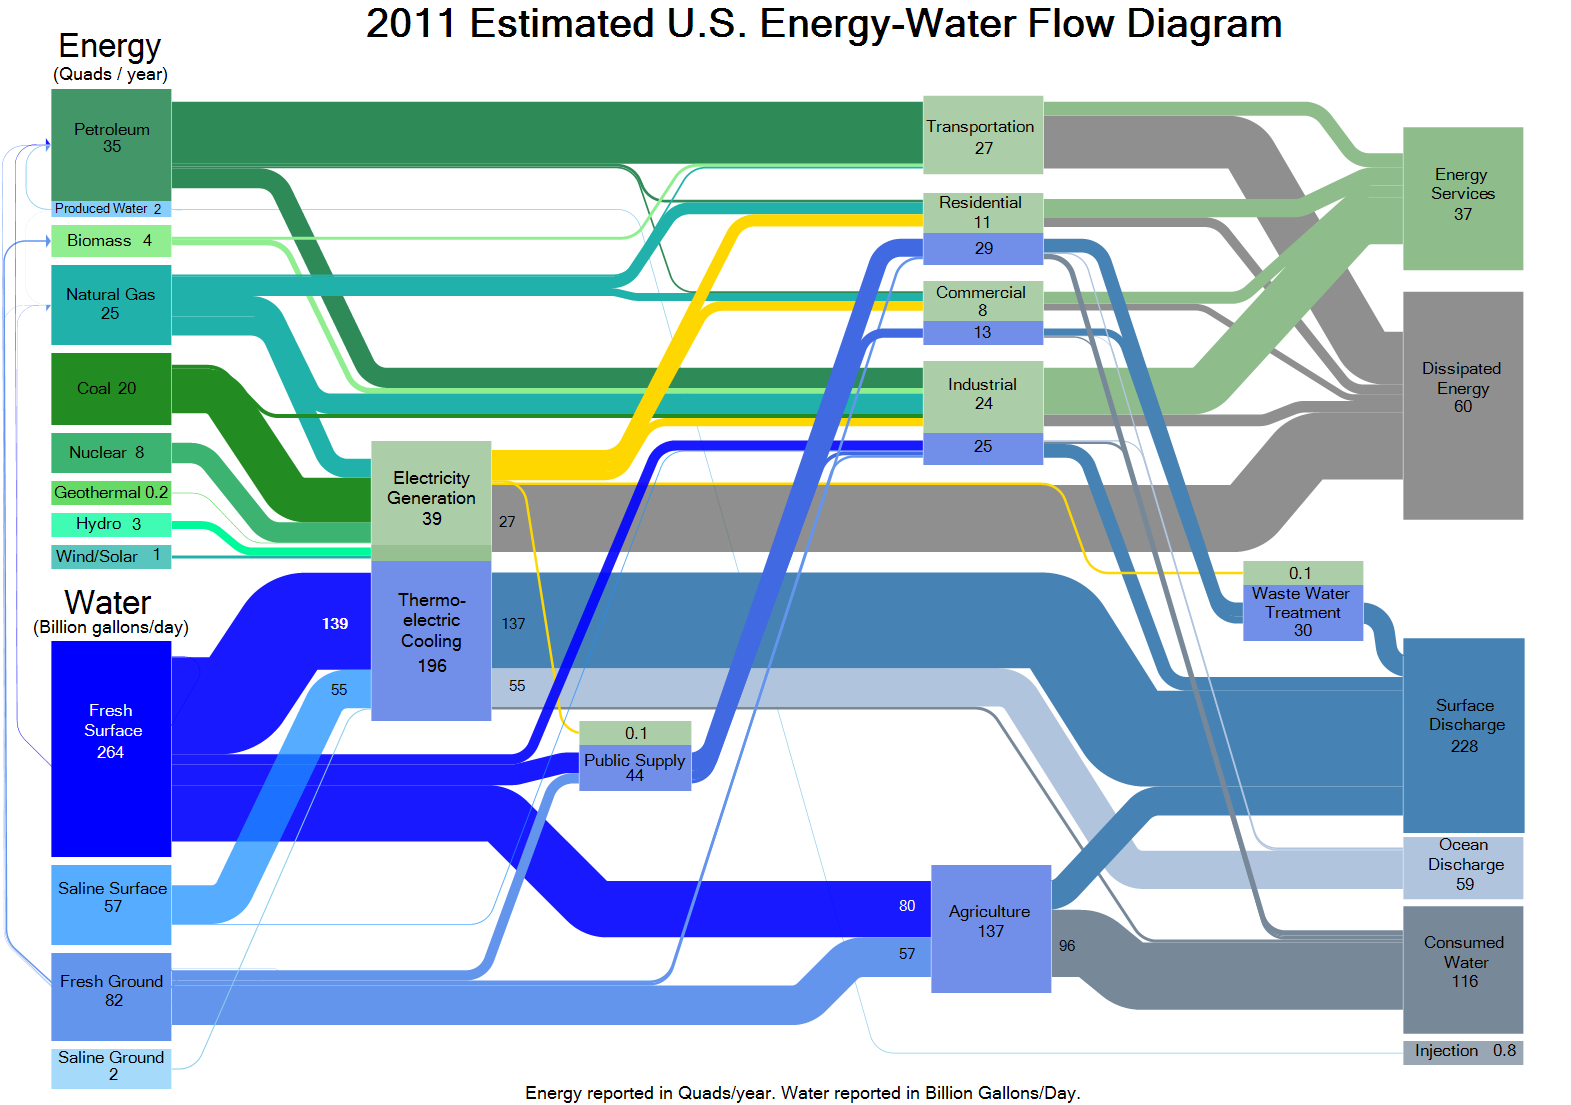
\includegraphics[width=6.5in]{extras18/energy-watersankey.png}
            \caption{U.S. water-energy flow chart for 2011 \cite{waterenergynexus}}
            \label{sankey}
            \end{figure}



\subsection{Direct}


Water conservation at the level of a building or energy system is straightforward---we want to use as little as possible to provide the services that we need. Direct water use is typically metered in gallons. 
Reducing direct water use in the built environment (Figure \ref{weu}) usually involves conservation in restrooms or shower facilities, in water used for heating or cooling (evaporative cooling can be a significant water consumer in commercial buildings here in the West), and in outdoor landscaping \cite{noauthor_2012-sd}. The EPA provides resources for choosing water-efficient fixtures for buildings  at \url{https://www.epa.gov/watersense}.

\begin{figure}[h]
\centering
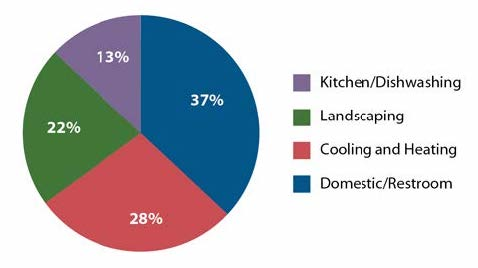
\includegraphics[width=2in]{extras18/weucb.jpg}
\caption{End uses of water in office buildings in the U.S. \cite{eGRIDsupportdoc2016}}
\label{weu}
\end{figure}



\subsection{Indirect}

A large portion of the water use that occurs due to human activity is hidden from our sight on a day-to-day basis. Indirect water use is also called `virtual water.'

\begin{quote}
    Water \textbf{withdrawal} describes the total amount of water withdrawn from a surface water or groundwater source. Measurements of this withdrawn water help evaluate demands from domestic, industrial and agricultural users. \cite{noauthor_2017-gg}
\end{quote}

\begin{quote}
Water \textbf{consumption} is the portion of the withdrawn water permanently lost from its source. This water is no longer available because it evaporated, got transpired or used by plants, or was consumed by people or livestock.
 \cite{noauthor_2017-gg}
\end{quote}

Some forms of power generation cooling systems might be extremely high in water withdrawn, with less being consumed (e.g. `once-through' cooling systems); other forms have very high consumption rates but much less water withdrawn (e.g. cooling towers). 


\subsection{Water factors}

As with emission factors, we can multiply out the quantity of electricity used by a water factor that  gives one number for the amount of water \textit{consumed} per unit of electrical energy (e.g. gal/MWh) and another number for the amount of water \textit{withdrawn} per unit of electrical energy (e.g. gal/MWh). There are a limited number of comprehensive studies that have considered the available data and existing studies on water use for electricity generation to come up with water withdrawal factors and water consumption factors, and there is significant variance in the actual possible values for those factors, so as we saw with emission factors, this type of analysis has inherent uncertainty. There are two very nice U.S.-focused reviews that provide estimates for both withdrawal and consumption factors: one published in 2012 comes from NREL researchers and focuses more on cooling system technologies \cite{Macknick2012-ol}; one published in 2013 comes from Western Water Assessment and NREL researchers and takes a life cycle perspective on electricity generation \cite{Meldrum2013-nk}.

\subsection{Embodied water}

Embodied (or you may also see the word `embedded') water indicates that the water use is not readily apparent but that it should be accounted for within the environmental analysis of some product or service. Water used to generate purchased power could be considered embedded water, as could water that was used to produce building components and items we purchase and use day-to-day.

\section{Nexus view}

The term \textbf{water-energy nexus} (or energy-water nexus) refers to the fact that energy and water systems are inextricably connected---water is used to generate electricity and provide energy services, and energy is used to extract, treat, and transport water. Constraints in water can lead to constraints in energy production, and vice versa \cite{waterenergynexus}.

Similarly, the climate is also affected by emissions and water use, so these interconnected systems are sometimes referred to together as the \textbf{water-energy-climate nexus} (or energy-water-climate nexus). Food production is critical to human health (and is also a contributor to many violent conflicts in the world), so the \textbf{food-energy-water nexus} (or water-food-energy; choose your preferred permutation) is an important area for interdisciplinary research \cite{Cai2018-zk}.


Overall, any of these ``nexus'' terms indicate that the person or organization is taking a systems-thinking perspective when talking about or analyzing the sectors that precede the word `nexus.'

% license
\bigskip

\noindent
\texttt{\footnotesize RESTRICTED PUBLIC LICENSE --- READ BEFORE SHARING. This is a draft version made available by Amanda D. Smith under a Creative Commons Attribution-NonCommercial-ShareAlike license. 
\href{https://creativecommons.org/licenses/by-nc-sa/4.0/}{CC BY-NC-SA 4.0}}

% references

\printbibliography

\end{document}